\documentclass[11pt,letterpaper]{article}
\usepackage[margin=1in]{geometry}
\usepackage{amsmath,amssymb,booktabs,array,graphicx,xcolor,listings,float}
\usepackage[hidelinks]{hyperref}
\usepackage{caption}
\captionsetup{font=small}
\setlength{\parskip}{5pt}
\setlength{\parindent}{1.2em}
\newcommand{\question}[1]{\noindent\textbf{Question:}\begin{quote}#1\end{quote}\noindent\textbf{Answer:}\par}
\lstset{basicstyle=\ttfamily\scriptsize,numbers=left,numberstyle=\tiny\color{gray},
 numbersep=7pt,breaklines=true,breakatwhitespace=false,columns=fullflexible,
 keepspaces=true,showstringspaces=false,tabsize=4,frame=none,
 keywordstyle=\bfseries,commentstyle=\itshape\color{black!65},
 aboveskip=8pt,belowskip=8pt}
% All numerical values are generated from measured round logs.

\title{CPEN 502 -- Assignment 1\\Part 2: Reinforcement Learning using a Look-Up-Table}
\author{Yujie Lin}
\date{\today}
\begin{document}
\maketitle
\section*{(2) LUT States and Actions}
\question{Please provide a description of your LUT in terms of the states and actions you chose to use, how or if they were quantized and the resulting total number of rows in the LUT.}
A robot extending \texttt{AdvancedRobot} was implemented in Java for classic Robocode 1.9.5.6. It learns a state--action value function using Q-learning and a look-up table (LUT). All reported results come from actual headless Robocode battles against the unmodified built-in \texttt{sample.SpinBot}; the source, round-level logs and trained tables accompany this report.

The continuous observations are reduced to five discrete variables. Energy is measured in Robocode energy units, and distances are measured in battlefield pixels. The bearing is the enemy's direction relative to the robot's current body heading, computed from its latest scanned position.
\begin{center}\small
\begin{tabular}{p{1.12in}cp{3.65in}}
\toprule
State variable & Bins & Quantization \\\midrule
Own energy & 3 & $[0,30)$, $[30,70)$, $[70,\infty)$ \\
Enemy energy & 3 & Same thresholds, using the latest scan \\
Enemy distance & 3 & $[0,200)$, $[200,400)$, $[400,\infty)$ \\
Relative bearing & 4 & Front: $[-45^\circ,45^\circ)$; right: $[45^\circ,135^\circ)$; back: $[135^\circ,180^\circ]\cup[-180^\circ,-135^\circ)$; left: $[-135^\circ,-45^\circ)$ \\
Near a wall & 2 & 1 if the robot centre is less than 80 pixels from any wall; otherwise 0 \\
\bottomrule
\end{tabular}
\end{center}
Thus, the state space has $3\times3\times3\times4\times2=216$ states. Each state has six available actions, giving
\[
\boxed{216\text{ state rows}\times6\text{ action columns}=1,296\text{ Q-values}.}
\]
Equivalently, a flattened table has \textbf{1,296 state--action rows}, each storing one scalar $Q(s,a)$. Both conventions describe the same LUT; no separate table entry is allocated for terminal states.

\newpage
\subsection*{Actions and Table Implementation}
Each decision selects one of the following macro-actions for 16 simulation ticks, unless the round terminates earlier. Movement uses asynchronous commands so radar and gun tracking continue while the robot moves.
\begin{center}\small
\begin{tabular}{clp{3.9in}}
\toprule
ID & Action & Command and firing behaviour \\\midrule
0 & Forward & Command 120 pixels forward; fire power 2 when ready. \\
1 & Backward & Command 120 pixels backward; fire power 2 when ready. \\
2 & Left arc & Command 120 pixels forward and $45^\circ$ left; fire power 2. \\
3 & Right arc & Command 120 pixels forward and $45^\circ$ right; fire power 2. \\
4 & Stop and fire low & Command zero movement and rotation; fire power 1. \\
5 & Stop and fire high & Command zero movement and rotation; fire power 3. \\
\bottomrule
\end{tabular}
\end{center}
The commands are replaced at the next decision, so the requested 120 pixels need not be completed. Stopping still obeys the simulator's deceleration. All actions use the same fixed aiming routine: point the gun at the latest observed enemy position and fire only when the gun is cool, the scan is at most four ticks old, the angular error is below 0.12 radians, and energy exceeds bullet power by 0.1. The LUT learns movement and firing mode; radar tracking and gun aiming are fixed support routines.

Writing the bin coordinates as $(e_o,e_n,d,b,w)$, the state and flat indices are
\[
s=((((e_o\cdot3+e_n)\cdot3+d)\cdot4+b)\cdot2+w),\qquad i=6s+a.
\]
All Q-values start at zero. The Q array requires $1,296\times8=10,368$ bytes, and a parallel integer visit-count array requires 5,184 bytes, excluding Java object overhead. Quantization therefore keeps the table small enough for the robot's data allowance.

\textbf{Consistency with Part 1.} The Java \texttt{CommonInterface} preserves the method names \texttt{load}, \texttt{save}, \texttt{train} and \texttt{output\_for} from the Python interface in Part 1. The input is a six-element vector containing the five state bins and an action. \texttt{output\_for} returns a scalar; \texttt{train(x,target)} returns the pre-update half squared error, as in Part 1. For the LUT it installs the supplied value directly; the RL controller first calculates $Q+\alpha(y-Q)$. This is semantic interface compatibility across languages, rather than a claim that the original Python class can be inserted into Java unchanged.

\textbf{Saving the learned table.} At the end of the final round, \texttt{save} writes all values and visit counts using \texttt{RobocodeFileOutputStream}. The big-endian file contains an 8-byte header and 1,296 $(\texttt{double},\texttt{int})$ entries, totalling \textbf{15,560 bytes}. \texttt{load} validates the header, dimensions and entries before replacing the table. CSV exports include every row, even entries with zero visits, for later neural-network training.

\textbf{Representation limits.} The table omits velocity, gun heat, absolute position and enemy motion. It also uses a possibly stale enemy scan. Different physical situations can therefore share one state. This is a practical approximation to a Markov state and limits any claim of convergence to an optimal Robocode policy.

\newpage
\section*{(3) Learning Performance}
\subsection*{Experimental Setup and Reward Generation}
Every condition was trained from a fresh zero LUT for \textbf{800 rounds per seed}, using seeds 0--4, followed by \textbf{200 evaluation rounds per seed}. The battlefield is $800\times600$, with one \texttt{sample.SpinBot} opponent, default gun cooling 0.1 and default inactivity setting. Battlefield initialization is randomized by the engine. Each condition uses the same five seed identifiers for Robocode's \texttt{RandomFactory} and the robot's independent action generator. Evaluation uses new seeds 10000--10004, sets $\epsilon=0$, disables learning and reloads the corresponding trained table.

There are seven conditions: Q-learning with intermediate rewards at $\epsilon\in\{0,0.1,0.3,0.6,1\}$; SARSA with intermediate rewards at $\epsilon=0.1$; and Q-learning with terminal-only rewards at $\epsilon=0.1$. An additional zero-LUT evaluation provides an untrained reference. In total, this is $7\times5\times(800+200)+5\times200=\textbf{36,000 rounds}$.

Both learners use $\alpha=0.1$ and $\gamma=0.95$. With $r$ the sum of rewards since the previous decision, Q-learning uses
\[
y_Q=r+\gamma\max_{a'}Q(s',a'),\qquad
Q(s,a)\leftarrow Q(s,a)+\alpha[y_Q-Q(s,a)].
\]
SARSA replaces the maximum with $Q(s',a')$, where $a'$ is the next action selected by the same $\epsilon$-greedy behaviour policy. The selected action is then actually executed. At a win or death, the final target is $y=r$ with \textbf{no bootstrap} and the last transition is updated exactly once. The terminal reward is $+10$ for a win and $-10$ for death.

For the intermediate-reward condition, event handlers additionally generate
\[
 r_{\rm hit}=D(p)/10,\qquad r_{\rm hit\ by\ bullet}=-D(p)/10,
 \qquad r_{\rm wall}=-0.2,
\]
where $D(p)=4p+\max(0,2(p-1))$ is the nominal damage of a bullet of power $p$. Bullet-hit rewards use nominal damage, which can exceed actual energy removed by a final hit. All events between decisions contribute to the pending reward; the terminal-only condition suppresses these intermediate terms. No separate reward is issued for firing, missing or colliding with a robot.

Discounting is \emph{per decision}, not per simulation tick; within a macro-action, event rewards are summed without extra temporal discount. A bullet landing after a later decision is credited to the action active when the event is received. This delayed-credit approximation is shared by all conditions.

\textbf{Measurement.} The primary outcome is the fraction of rounds producing a WinEvent; deaths, including simultaneous deaths, count as non-wins. This avoids comparisons of differently scaled rewards. Curves show a trailing 50-round win rate averaged over five seeds; shading is $\pm1$ sample standard deviation across seeds. Evaluation bars use the same seed-level mean and standard deviation over five 200-round blocks. These are variability bands, not confidence intervals. All frozen evaluations were checked to leave the binary LUT unchanged.

\newpage
\subsection*{(3a) Learning Progress and Convergence}
\question{Draw a graph of a parameter that reflects a measure of progress of learning and comment on the convergence of learning of your robot.}
Win rate was selected as the main progress measure. Figure~\ref{fig:learning} also shows the mean absolute temporal-difference error per round and the cumulative number of visited state--action pairs. The TD statistic is averaged over updates within a round, then over the trailing 50 rounds and the five seeds.
\begin{figure}[H]\centering
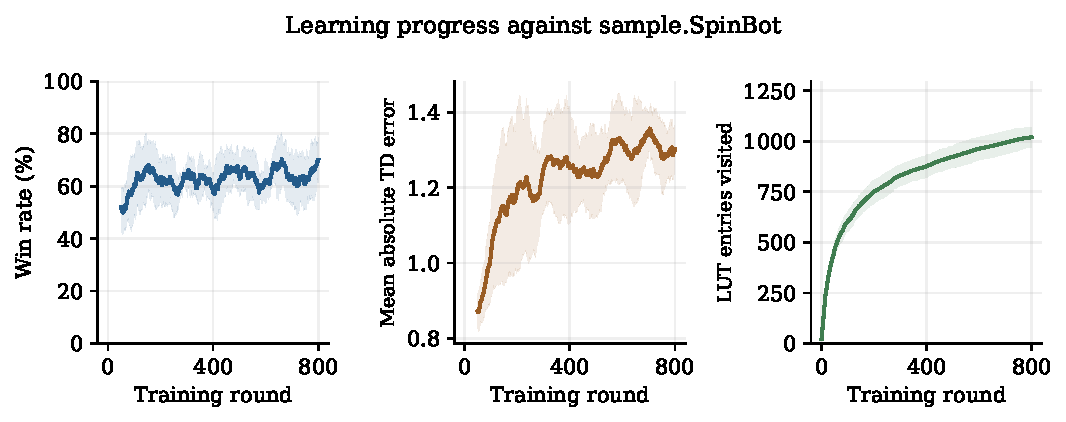
\includegraphics[width=\linewidth,height=2.8in,keepaspectratio]{figures/learning.pdf}
\caption{Q-learning with intermediate rewards and $\epsilon=0.1$. Trailing 50-round win rate and TD error; coverage uses unsmoothed cumulative visit counts. Shading indicates one standard deviation across five seeds.}\label{fig:learning}
\end{figure}
The mean win rate changes from 56.2\% in rounds 1--100 to 65.4\% in rounds 701--800. Frozen greedy evaluation achieves 64.6\% $\pm$ 8.2 percentage points, compared with 54.8\% $\pm$ 1.8 for an untrained zero LUT with random tie-breaking on the same evaluation seed identifiers. Thus, the learned policy exceeds that untrained reference by 9.8 percentage points on average.

Coverage reaches a mean of 1019.8 of 1,296 entries (78.7\%). Mean absolute TD error averaged over the first and last 100 rounds is 0.949 and 1.290, respectively. The curve provides evidence of learning, but the remaining fluctuations and incomplete coverage do not support declaring full value-function convergence within 800 rounds.\par

Constant $\alpha$, continuing exploration, randomized initial conditions and the compressed observation space all permit persistent fluctuations. A plateau in win rate is evidence of a performance level over this training budget, rather than proof of convergence of every Q-value. Mean absolute TD error need not approach zero under stochastic transitions and rewards, even if the estimated values have stabilized.

\newpage
\subsection*{(3b) On-Policy versus Off-Policy Learning}
\question{Using your robot, show a graph comparing the performance of your robot using on-policy learning vs off-policy learning.}
Q-learning is the off-policy method, and SARSA is the on-policy method. Both use intermediate rewards, $\epsilon=0.1$, the same state/action representation and the same training budget. Only the bootstrap target changes:
\[
\underbrace{r+\gamma\max_{a'}Q(s',a')}_{\text{Q-learning: greedy target policy}}
\quad\text{versus}\quad
\underbrace{r+\gamma Q(s',a'_{\epsilon\text{-greedy}})}_{\text{SARSA: behaviour-policy target}}.
\]
\begin{figure}[H]\centering
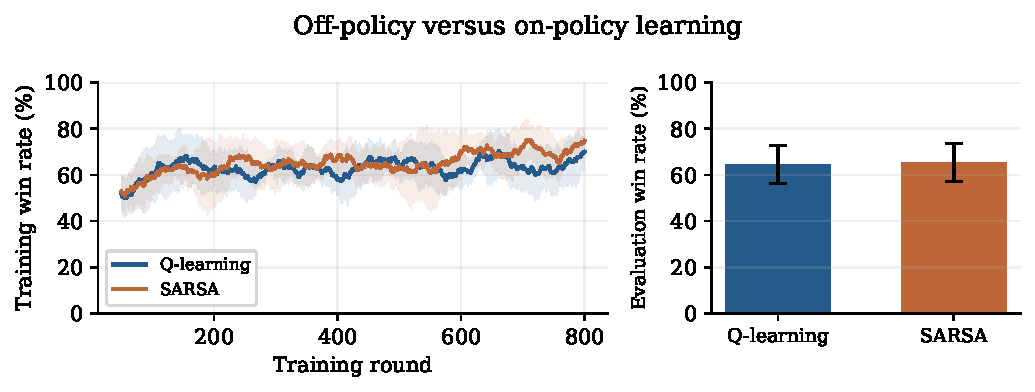
\includegraphics[width=.88\linewidth]{figures/policy.pdf}
\caption{On-policy and off-policy comparison. Left: measured training win rate. Right: frozen greedy evaluation after 800 training rounds. Shading and error bars are one standard deviation across seeds.}\label{fig:policy}
\end{figure}
\begin{center}\small\begin{tabular}{lrrr}
\toprule
Method & First 100 (\%) & Last 100 (\%) & Evaluation (\%) \\
\midrule
Q-learning & 56.2 & 65.4 & $64.6 \pm 8.2$ \\
SARSA & 56.0 & 71.2 & $65.4 \pm 8.3$ \\
\bottomrule
\end{tabular}
\end{center}
The observed greedy evaluation win rate is 64.6\% for Q-learning and 65.4\% for SARSA. SARSA is 0.8 percentage points higher on average. Seed-level paired SARSA-minus-Q-learning differences range from -18.5 to 13.0 percentage points. This range shows why the five-seed distribution matters: the average ordering alone does not establish a reliable advantage across runs.\par

Both algorithms explore with the same probability. Q-learning evaluates a greedy continuation, while SARSA accounts for the sampled exploratory continuation. This can make SARSA sensitive to the risks of exploratory actions, but does not guarantee higher performance.

Evaluation sets $\epsilon=0$ for both methods. Since SARSA was trained to evaluate an $\epsilon$-greedy policy, its training curve is also relevant. Shared seed identifiers control the starting random streams; divergent actions subsequently produce different trajectories.

\newpage
\subsection*{(3c) Terminal-Only versus Intermediate Rewards}
\question{Implement a version of your robot that assumes only terminal rewards and show \& compare its behaviour with one having intermediate rewards.}
The terminal-only robot receives zero reward during a round and $+10/-10$ at its end. The intermediate-reward robot receives the same terminal reward plus the bullet and wall terms defined above. Both use Q-learning, $\epsilon=0.1$, $\alpha=0.1$ and $\gamma=0.95$.
\begin{figure}[H]\centering
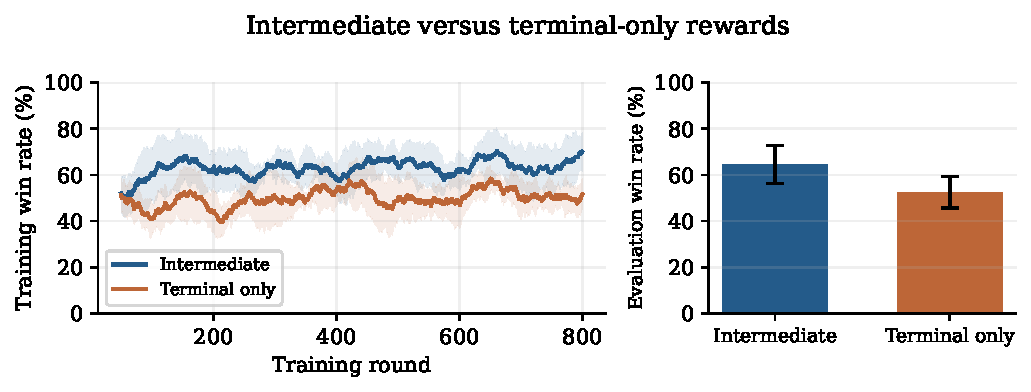
\includegraphics[width=.90\linewidth]{figures/rewards.pdf}
\caption{Reward-design comparison. Training and frozen evaluation win rates use a common outcome measure, rather than comparing the different reward totals. Error bars and shading show one standard deviation across seeds.}\label{fig:rewards}
\end{figure}
\begin{center}\small\begin{tabular}{lrr}
\toprule
Metric & Intermediate & Terminal only \\
\midrule
Evaluation win rate (\%) & $64.6 \pm 8.2$ & $52.4 \pm 6.7$ \\
Nominal bullet damage dealt per round & 84.5 & 78.9 \\
Nominal bullet damage received per round & 53.0 & 58.4 \\
Wall-hit events per round & 6.2 & 11.6 \\
Bullet hit rate (\%) & 26.4 & 25.4 \\
Simulation ticks per round & 457.1 & 454.5 \\
\bottomrule
\end{tabular}
\end{center}
Intermediate rewards produce a mean evaluation win rate of 64.6\%, versus 52.4\% with terminal-only rewards, a difference of 12.2 percentage points. Under greedy evaluation, the intermediate-reward robot records 6.2 wall-hit events per round compared with 11.6, so it makes fewer wall contacts on average. It deals 84.5 rather than 78.9 nominal bullet damage per round. These measurements describe the learned behaviour in this experiment; they do not imply that the shaping guarantees collision avoidance or higher win rates in other settings.\par

Terminal-only learning must propagate final outcomes backward through repeated visits. Intermediate events give more frequent shooting and wall feedback. The behaviour table measures damage and collisions directly.

These terms are not potential-based shaping and also change the optimized objective. The observed advantage is conditional on this opponent and training budget.

\newpage
\section*{(4) Exploration}
\subsection*{(4a) Performance at Different Exploration Rates}
\question{Compare training performance using different values of $e$ including no exploration at all. Provide graphs of the measured performance of your tank vs $e$.}
At each decision, the robot chooses uniformly from all six actions with probability $e$ and chooses a greedy action with probability $1-e$. Thus, with a unique maximizer, the greedy action has probability $1-e+\frac{e}{6}$ and each other action has probability $\frac{e}{6}$. Exploration can select the greedy action too.

Five constant rates, $e=0,0.1,0.3,0.6,1.0$, were tested using Q-learning and intermediate rewards. All start with a zero LUT, and ties between maximizing actions are broken uniformly at random in every condition. Therefore, $e=0$ removes \emph{explicit} exploration but still permits random actions when Q-values tie. At initialization all six actions tie; this differs from fixing the first action on every tie and avoids an arbitrary action-order bias.
\begin{figure}[H]\centering
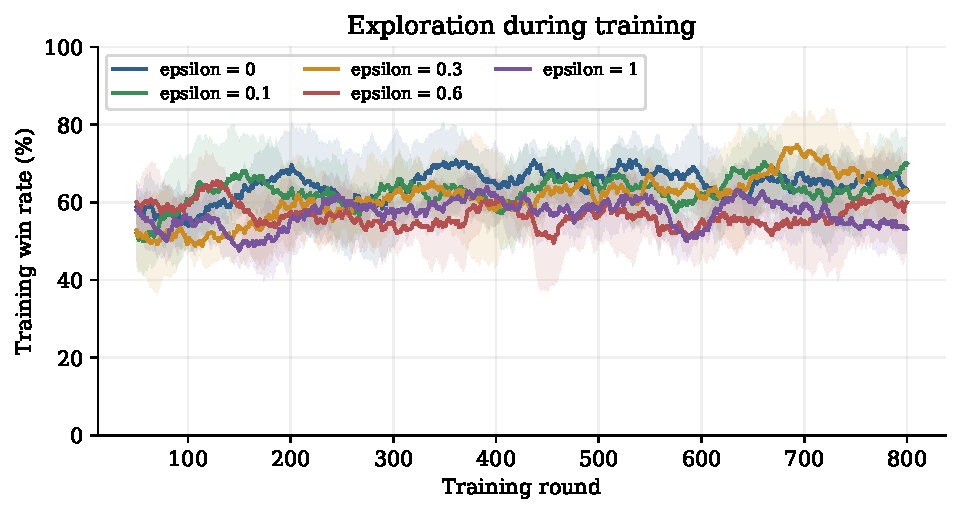
\includegraphics[width=.84\linewidth]{figures/epsilon_curves.pdf}
\caption{Training curves for five fixed exploration probabilities. Each line is the mean trailing 50-round win rate across five independent training seeds; shading is one standard deviation.}\label{fig:epsilon_curves}
\end{figure}
Across the full training budget, the highest mean training win rate is 64.1\% at $e=0$. The corresponding mean for $e=1$ is 57.0\%. The curves show the effect of the behaviour policy while learning, including its exploratory moves; they should not be read as evaluations of an exploration-free policy.\par

At $e=1$, actions remain uniformly random throughout training even though Q-learning continues updating the table. Its training win rate therefore measures random behaviour, while its subsequent $e=0$ evaluation tests the learned greedy values. The two quantities answer different questions and need not agree.

\newpage
\subsection*{Performance versus Exploration Probability}
\begin{figure}[H]\centering
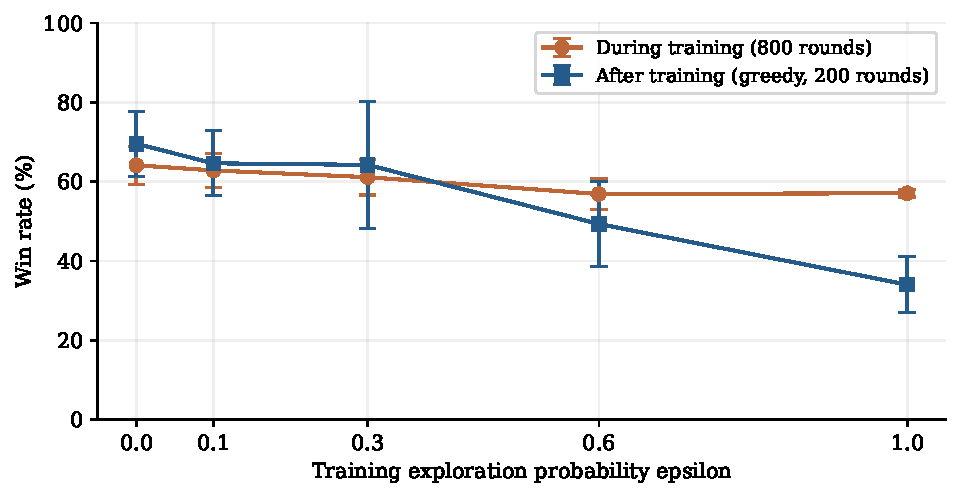
\includegraphics[width=.9\linewidth]{figures/epsilon_summary.pdf}
\caption{Performance versus the exploration rate used during training. Orange: average win rate over all 800 training rounds. Blue: frozen greedy evaluation over 200 new rounds. Error bars are one standard deviation across five seeds; connecting lines guide the eye between tested rates.}\label{fig:epsilon_summary}
\end{figure}
\begin{center}\small\begin{tabular}{lrrr}
\toprule
Training $e$ & All training (\%) & Last 100 (\%) & Greedy evaluation (\%) \\
\midrule
0 & 64.1 & 64.0 & $69.5 \pm 8.2$ \\
0.1 & 62.8 & 65.4 & $64.6 \pm 8.2$ \\
0.3 & 61.1 & 65.6 & $64.2 \pm 16.0$ \\
0.6 & 56.9 & 59.2 & $49.3 \pm 10.7$ \\
1 & 57.0 & 53.6 & $34.0 \pm 7.0$ \\
\bottomrule
\end{tabular}
\end{center}
The highest observed greedy evaluation mean is 69.5\% at training $e=0$, while $e=0.1$ yields 64.6\%. At training $e=1$, the learned greedy policy obtains 34.0\%, compared with 57.0\% for its random training behaviour. Broad exploration alone therefore did not yield the strongest greedy policy within this finite budget. The $e=0$ result is also informative: zero initialization and random tie-breaking permit initial action diversity even without explicitly random exploration.\par

The best observed rate is conditional on this opponent, reward function, quantization and 800-round budget. A constant high exploration rate can lower online performance through repeated suboptimal moves; zero explicit exploration can exploit useful early estimates but can also neglect actions once ties disappear. The experiment does not establish a universally optimal exploration rate. No decaying schedule was tested.

\newpage
\subsection*{Implementation Validation and Reproducibility}
Checks passed for all 1,296 index/decode mappings, the half squared error interface, TD arithmetic, terminal updates, greedy action choice, uniform exploration, unbiased tie-breaking, saved Q-values/visit counts, file dimensions and rejection of corrupt files. Every recorded condition contains the expected round count. Evaluations leave the trained binary LUT byte-identical. The robot source, controller, experiment drivers and analysis script are included in the appendix; all raw logs, seed-level tables and trained LUTs are included in the accompanying package. JVM version, scheduling and skipped simulation turns can affect exact reruns.

\textbf{Preparing for the neural replacement.} A later network can learn from the exported state--action vectors and unrestricted real Q targets. The original XOR network's two inputs and bounded sigmoid output must be adapted to this six-coordinate input and Q-value scale. Saving the LUT provides supervised examples, while the common method names preserve the controller's conceptual interface.

\section*{References}
\begin{enumerate}
\item R. S. Sutton and A. G. Barto. \emph{Reinforcement Learning: An Introduction}, 2nd ed., MIT Press, 2018, Sections 6.4--6.5. \url{https://www.andrew.cmu.edu/course/10-703/textbook/BartoSutton.pdf}
\item Robocode project. Classic Robocode 1.9.5.6 distribution and sample robot source. \url{https://github.com/robo-code/robocode/releases/tag/VER_1_9_5_6}
\item Robocode project. \emph{AdvancedRobot}, \emph{Rules}, \emph{RobocodeEngine} and \emph{BattleSpecification} API documentation. The public documentation is version 1.10.0; the implementation was compiled and executed against 1.9.5.6. \url{https://robocode.sourceforge.io/docs/robocode/}
\end{enumerate}
The learning equations follow reference 1. The engine, sample opponent, event API and bullet-damage rule are from references 2--3. All tables and graphs in this report were calculated from the accompanying Robocode runs; they are not adapted from reference results.

\newpage
\appendix
\newgeometry{left=.85in,right=.85in,top=.85in,bottom=.85in}
\lstset{basicstyle=\ttfamily\fontsize{7.5}{8.6}\selectfont}
\section*{Appendix A Source Code}
\subsection*{A1 CommonInterface.java}
\begin{lstlisting}[language=Java]
package lutbot;
import java.io.IOException;
/** Same method names and scalar-regression semantics as Part 1. */
public interface CommonInterface {
    void load(String path) throws IOException;
    void save(String path) throws IOException;
    double train(double[] x, double target);
    double output_for(double[] x);
}
\end{lstlisting}
\subsection*{A2 LUT.java}
\begin{lstlisting}[language=Java]
package lutbot;
import java.io.*;
import java.util.Random;
import robocode.RobocodeFileOutputStream;
/** Input: five quantized state coordinates followed by action. */
public class LUT implements CommonInterface {
    public static final int[] BINS = {3, 3, 3, 4, 2, 6};
    public static final int STATES = 216, ACTIONS = 6, SIZE = 1296;
    private final double[] q = new double[SIZE];
    private final int[] visits = new int[SIZE];
    public static int index(double[] x) {
        if (x.length != BINS.length) throw new IllegalArgumentException("6 coordinates required");
        int n = 0;
        for (int i = 0; i < x.length; i++) {
            int b = (int)x[i];
            if (x[i] != b || b < 0 || b >= BINS[i])
                throw new IllegalArgumentException("Invalid bin");
            n = n * BINS[i] + b;
        }
        return n;
    }
    public double output_for(double[] x) { return q[index(x)]; }
    public double train(double[] x, double target) {
        if (!Double.isFinite(target)) throw new IllegalArgumentException("Nonfinite target");
        int i = index(x);
        double error = target - q[i];
        q[i] = target; // RL controller already applies alpha.
        visits[i]++;
        return 0.5 * error * error;
    }
    public double value(int s, int a) { return q[s * ACTIONS + a]; }
    public double max(int s) {
        double m = Double.NEGATIVE_INFINITY;
        for (int a = 0; a < ACTIONS; a++) m = Math.max(m, value(s,a));
        return m;
    }
    public int choose(int s, double epsilon, Random rng) {
        if (rng.nextDouble() < epsilon) return rng.nextInt(ACTIONS);
        double best = max(s);
        int n = 0, chosen = 0;
        for (int a = 0; a < ACTIONS; a++)
            if (value(s,a) == best && rng.nextInt(++n) == 0) chosen = a;
        return chosen; // Uniform random tie-breaking, including epsilon=0.
    }
    public double update(int s, int a, double target, double alpha) {
        double[] x = decode(s * ACTIONS + a);
        double delta = target - output_for(x);
        train(x, output_for(x) + alpha * delta);
        return delta;
    }
    public static double[] decode(int n) {
        double[] x = new double[6];
        for (int i=5; i>=0; i--) { x[i] = n % BINS[i]; n /= BINS[i]; }
        return x;
    }
    public int covered() {
        int n=0; for (int v: visits) if (v>0) n++; return n;
    }
    public void save(String path) throws IOException {
        try (DataOutputStream out = new DataOutputStream(new RobocodeFileOutputStream(path))) {
            out.writeInt(0x4c555432); out.writeInt(SIZE);
            for (int i=0; i<SIZE; i++) { out.writeDouble(q[i]); out.writeInt(visits[i]); }
        }
    }
    public void load(String path) throws IOException {
        double[] temp = new double[SIZE]; int[] count = new int[SIZE];
        try (DataInputStream in = new DataInputStream(new FileInputStream(path))) {
            if (in.readInt()!=0x4c555432 || in.readInt()!=SIZE)
                throw new IOException("LUT format mismatch");
            for (int i=0; i<SIZE; i++) {
                temp[i]=in.readDouble(); count[i]=in.readInt();
                if (!Double.isFinite(temp[i]) || count[i]<0) throw new IOException("Invalid entry");
            }
            if (in.read()!=-1) throw new IOException("Trailing bytes");
        }
        System.arraycopy(temp,0,q,0,SIZE); System.arraycopy(count,0,visits,0,SIZE);
    }
}
\end{lstlisting}
\newpage
\subsection*{A3 LearningTank.java}
\begin{lstlisting}[language=Java]
package lutbot;
import robocode.*;
import robocode.util.Utils;
import java.io.*;
import java.util.*;

/** Six 16-tick macro-actions; only one opponent is supported. */
public class LearningTank extends AdvancedRobot {
    private static LUT lut;
    private static Random rng;
    private static Properties config;
    private double epsilon;
    private boolean sarsa, intermediate, learning;
    private int state=-1, action, steps, wallHits, shots, hits;
    private long nextDecision;
    private double pending, totalReward, tdAbs, dealt, received;
    private double enemyX, enemyY, enemyEnergy=100, distance=500;
    private long lastScan=-100;
    private boolean finished;
    private static String cfg(String k, String fallback) {
        return config.getProperty(k,fallback);
    }
    public void run() {
        if (getRoundNum()==0 || lut==null) {
            config = new Properties();
            try (InputStream in=new FileInputStream(getDataFile("config.properties"))) {
                config.load(in);
            } catch (IOException e) { out.println("Using default config: "+e); }
            lut = new LUT();
            rng = new Random(Long.parseLong(cfg("seed","0")));
            if (Boolean.parseBoolean(cfg("resume","false"))) {
                try { lut.load(getDataFile("trained.lut").getPath()); }
                catch(IOException e) { throw new IllegalStateException("Cannot resume",e); }
            }
        }
        if (getRoundNum()==0) out.println("CONFIG "+config);
        epsilon=Double.parseDouble(cfg("epsilon","0.1"));
        sarsa=cfg("algorithm","q").equals("sarsa");
        intermediate=Boolean.parseBoolean(cfg("intermediate","true"));
        learning=Boolean.parseBoolean(cfg("learning","true"));
        setAdjustGunForRobotTurn(true);
        setAdjustRadarForGunTurn(true);
        setAdjustRadarForRobotTurn(true);
        setTurnRadarRight(Double.POSITIVE_INFINITY);
        while (true) {
            if (lastScan>=0) {
                if (state<0 || getTime()>=nextDecision) decide();
                aimAndFire();
            }
            if (getTime()-lastScan>4)
                setTurnRadarRight(Double.POSITIVE_INFINITY);
            execute();
        }
    }
    private int energyBin(double e) { return e<30 ? 0 : e<70 ? 1 : 2; }
    private int observe() {
        double d=Math.hypot(enemyX-getX(),enemyY-getY());
        int db=d<200 ? 0 : d<400 ? 1 : 2;
        double absolute=Math.atan2(enemyX-getX(),enemyY-getY());
        double b=Utils.normalAbsoluteAngle(absolute-getHeadingRadians()+Math.PI/4);
        int bearing=(int)(b/(Math.PI/2));
        double wall=Math.min(Math.min(getX(),getBattleFieldWidth()-getX()),
                             Math.min(getY(),getBattleFieldHeight()-getY()));
        double[] x={energyBin(getEnergy()),energyBin(enemyEnergy),db,bearing,wall<80?1:0,0};
        return LUT.index(x)/LUT.ACTIONS;
    }
    private void decide() {
        int nextState=observe();
        int nextAction=lut.choose(nextState,epsilon,rng);
        if (state>=0) {
            double boot=sarsa ? lut.value(nextState,nextAction) : lut.max(nextState);
            update(pending+0.95*boot);
        }
        state=nextState; action=nextAction; pending=0;
        nextDecision=getTime()+16;
        // Reset old commands before issuing the selected macro-action.
        setAhead(0); setTurnRight(0);
        if (action==0) setAhead(120);
        if (action==1) setBack(120);
        if (action==2) { setAhead(120); setTurnLeft(45); }
        if (action==3) { setAhead(120); setTurnRight(45); }
        // Actions 4/5 stop and use a different bullet power.
    }
    private void update(double target) {
        if (!learning) return;
        tdAbs+=Math.abs(lut.update(state,action,target,0.1)); steps++;
    }
    private void aimAndFire() {
        double aim=Math.atan2(enemyX-getX(),enemyY-getY());
        setTurnGunRightRadians(Utils.normalRelativeAngle(aim-getGunHeadingRadians()));
        if (state>=0 && getTime()-lastScan<=4 && getGunHeat()==0
                && Math.abs(Utils.normalRelativeAngle(aim-getGunHeadingRadians()))<0.12) {
            double power=action==4 ? 1 : action==5 ? 3 : 2;
            if (getEnergy()>power+0.1 && setFireBullet(power)!=null) shots++;
        }
    }
    public void onScannedRobot(ScannedRobotEvent e) {
        double abs=getHeadingRadians()+e.getBearingRadians();
        distance=e.getDistance();
        enemyX=getX()+Math.sin(abs)*distance;
        enemyY=getY()+Math.cos(abs)*distance;
        enemyEnergy=e.getEnergy(); lastScan=getTime();
        double turn=Utils.normalRelativeAngle(abs-getRadarHeadingRadians());
        setTurnRadarRightRadians(turn==0 ? 0.02 : 2*turn);
    }
    private void reward(double r) {
        if (state>=0 && !finished) { pending+=r; totalReward+=r; }
    }
    public void onBulletHit(BulletHitEvent e) {
        double p=e.getBullet().getPower(), damage=4*p+Math.max(0,2*(p-1));
        dealt+=damage; hits++;
        if (intermediate) reward(damage/10.0);
    }
    public void onHitByBullet(HitByBulletEvent e) {
        double p=e.getBullet().getPower(), damage=4*p+Math.max(0,2*(p-1));
        received+=damage;
        if (intermediate) reward(-damage/10.0);
    }
    public void onHitWall(HitWallEvent e) {
        wallHits++; if (intermediate) reward(-0.2);
    }
    public void onWin(WinEvent e) { finish(1); }
    public void onDeath(DeathEvent e) { finish(0); }
    private void finish(int outcome) {
        if (finished) return;
        reward(outcome==1 ? 10 : outcome==0 ? -10 : 0);
        if (state>=0) update(pending); // Terminal target has NO bootstrap.
        finished=true;
        try {
            if (getRoundNum()==getNumRounds()-1)
                lut.save(getDataFile("trained.lut").getPath());
            try (PrintStream out=new PrintStream(new RobocodeFileOutputStream(
                        getDataFile("metrics.csv").getPath(),getRoundNum()!=0))) {
                if (getRoundNum()==0) out.println("round,outcome,reward,mean_abs_td,updates,coverage,shots,hits,dealt,received,wall_hits,ticks");
                out.printf(Locale.US,"%d,%d,%.6f,%.6f,%d,%d,%d,%d,%.3f,%.3f,%d,%d%n",
                    getRoundNum()+1,outcome,totalReward,steps==0?0:tdAbs/steps,
                    steps,lut.covered(),shots,hits,dealt,received,wallHits,getTime());
            }
        } catch(IOException e) { throw new IllegalStateException("Persistence failed",e); }
    }
}
\end{lstlisting}
\newpage
\subsection*{A4 RunBattle.java}
\begin{lstlisting}[language=Java]
import robocode.control.*;
import robocode.control.events.*;
import java.io.*;
/** Usage: RunBattle ROBOCODE_HOME ROUNDS SEED */
public class RunBattle {
    public static void main(String[] args) {
        System.setProperty("java.awt.headless","true");
        RandomFactory.setRandom(new java.util.Random(Long.parseLong(args[2])));
        RobocodeEngine engine=new RobocodeEngine(new File(args[0]));
        engine.setVisible(false);
        engine.addBattleListener(new BattleAdaptor() {
            public void onBattleError(BattleErrorEvent e) { System.err.println(e.getError()); }
            public void onBattleCompleted(BattleCompletedEvent e) {
                for (robocode.BattleResults r:e.getSortedResults())
                    System.out.println(r.getTeamLeaderName()+" score="+r.getScore()+" wins="+r.getFirsts());
            }
        });
        RobotSpecification[] robots=engine.getLocalRepository("lutbot.LearningTank*,sample.SpinBot");
        if (robots.length!=2) throw new IllegalStateException("Expected two robots, got "+robots.length);
        engine.runBattle(new BattleSpecification(Integer.parseInt(args[1]),
                          new BattlefieldSpecification(800,600),robots),true);
        engine.close(); System.exit(0);
    }
}
\end{lstlisting}
\newpage
\subsection*{A5 LUTChecks.java}
\begin{lstlisting}[language=Java]
import lutbot.LUT;
import java.io.*;
import java.nio.file.*;
import java.util.*;
/** Deterministic checks of LUT indexing, TD arithmetic, policy and persistence. */
public class LUTChecks {
    private static void check(boolean ok, String label) {
        if (!ok) throw new AssertionError(label);
    }
    public static void main(String[] args) throws Exception {
        LUT q=new LUT();
        for(int i=0;i<LUT.SIZE;i++) check(LUT.index(LUT.decode(i))==i,"index round-trip");
        double[] x=LUT.decode(0);
        check(q.train(x,2)==2 && q.output_for(x)==2,"Part 1 error semantics");
        check(q.update(0,0,10,0.1)==8 && Math.abs(q.value(0,0)-2.8)<1e-12,"TD update");
        q.train(LUT.decode(6),5); q.train(LUT.decode(7),1);
        // With r=2 and gamma=.95: Q target=6.75, SARSA(a'=1) target=2.95.
        double qTarget=2+.95*q.max(1), sTarget=2+.95*q.value(1,1);
        check(Math.abs(qTarget-6.75)<1e-12 && Math.abs(sTarget-2.95)<1e-12,"bootstrap targets");
        q.update(0,0,-10,1);
        check(q.value(0,0)==-10,"terminal target without bootstrap");
        Random rng=new Random(5);
        for(int i=0;i<1000;i++) check(q.choose(1,0,rng)==0,"greedy policy");
        int[] n=new int[6]; for(int i=0;i<60000;i++) n[q.choose(1,1,rng)]++;
        for(int v:n) check(v>9500 && v<10500,"uniform exploration");
        LUT tied=new LUT(); Arrays.fill(n,0);
        for(int i=0;i<60000;i++) n[tied.choose(0,0,rng)]++;
        for(int v:n) check(v>9500 && v<10500,"unbiased greedy ties");
        Path file=Files.createTempFile("lut-check",".bin");
        LUT restored=new LUT(); restored.load(args[0]);
        try (DataInputStream in=new DataInputStream(new FileInputStream(args[0]))) {
            check(in.readInt()==0x4c555432 && in.readInt()==1296,"saved header");
            int covered=0;
            for(int i=0;i<LUT.SIZE;i++) {
                double expected=in.readDouble(); int count=in.readInt();
                check(expected==restored.output_for(LUT.decode(i)),"saved values");
                if(count>0) covered++;
            }
            check(covered==restored.covered(),"saved visits");
        }
        check(Files.size(Paths.get(args[0]))==15560,"binary size");
        double previous=restored.value(1,0);
        Files.write(file,new byte[]{0,1,2});
        try {restored.load(file.toString()); throw new AssertionError("corruption accepted");}
        catch(IOException expected) {}
        check(restored.value(1,0)==previous,"failed load leaves model intact");
        try {LUT.index(new double[]{3,0,0,0,0,0}); throw new AssertionError("invalid bin accepted");}
        catch(IllegalArgumentException expected) {}
        Files.delete(file);
        System.out.println("PASS: indexing, error semantics, TD targets, terminal update, epsilon policy, tie breaking, save/load, corrupt-file rejection");
    }
}
\end{lstlisting}
\newpage
\subsection*{A6 run\_experiments.py}
\begin{lstlisting}[language=Python]
"""Run real Robocode battles. No synthetic result generation.
Requires Java 17 and a classic Robocode 1.9.5.6 installation.
Compile src first (README). Run: python run_experiments.py --home PATH
"""
import argparse, concurrent.futures, csv, json, pathlib, shutil, subprocess, time
ROOT = pathlib.Path(__file__).resolve().parent
CONDITIONS = [("q_dense_e0", "q", True, 0.0),
              ("q_dense_e01", "q", True, 0.1),
              ("q_dense_e03", "q", True, 0.3),
              ("q_dense_e06", "q", True, 0.6),
              ("q_dense_e1", "q", True, 1.0),
              ("sarsa_dense_e01", "sarsa", True, 0.1),
              ("q_terminal_e01", "q", False, 0.1)]
JAVA_FLAGS = ["-Xmx384m", "-Djava.security.manager=allow",
              "-Dsun.reflect.noInflation=true",
              "--add-opens=java.base/java.lang=ALL-UNNAMED",
              "--add-opens=java.base/java.lang.reflect=ALL-UNNAMED",
              "--add-opens=java.base/sun.net.www.protocol.jar=ALL-UNNAMED"]
def one_seed(seed, args):
    home = (ROOT / "work" / f"seed{seed}").resolve()
    if home.exists(): shutil.rmtree(home)
    shutil.copytree(args.home, home)
    data = home / "robots/lutbot/LearningTank.data"
    data.mkdir(parents=True, exist_ok=True)
    outdir = ROOT / "results"
    outdir.mkdir(exist_ok=True)
    for name, algorithm, dense, epsilon in CONDITIONS:
        (home/'robots/robot.database').unlink(missing_ok=True)
        prefix = outdir / f"{name}_seed{seed}"
        for phase, rounds in [("train",args.rounds),("eval",args.evaluation)]:
            for f in ["metrics.csv", "config.properties"]:
                (data/f).unlink(missing_ok=True)
            if phase=="train": (data/"trained.lut").unlink(missing_ok=True)
            config = dict(seed=seed if phase=="train" else 10000+seed,
                          epsilon=epsilon if phase=="train" else 0,
                          algorithm=algorithm, intermediate=str(dense).lower(),
                          learning=str(phase=="train").lower(),
                          resume=str(phase=="eval").lower())
            (data/"config.properties").write_text("".join(f"{k}={v}\n" for k,v in config.items()))
            runner = pathlib.Path(args.runner).resolve()
            import os
            cp = str(home/"libs/robocode.jar") + os.pathsep + str(runner)
            cmd = ["java"]+JAVA_FLAGS+["-cp",cp,"RunBattle",str(home),str(rounds),
                                      str(config["seed"])]
            t=time.time()
            with open(str(prefix)+f"_{phase}.log","w") as log:
                subprocess.run(cmd,stdout=log,stderr=subprocess.STDOUT,check=True,timeout=1800,cwd=home)
            rows=list(csv.DictReader((data/"metrics.csv").open()))
            if len(rows)!=rounds or any(r['outcome'] not in ('0','1') for r in rows):
                raise RuntimeError(f"Incomplete battle: {name} seed {seed}")
            logtext=pathlib.Path(str(prefix)+f"_{phase}.log").read_text()
            if any(x in logtext for x in ('Exception','Preventing','SYSTEM:')):
                raise RuntimeError(f"Engine/robot failure: {prefix}_{phase}.log")
            shutil.copy2(data/"metrics.csv",str(prefix)+f"_{phase}.csv")
            if phase=="train": shutil.copy2(data/"trained.lut",str(prefix)+".lut")
            else:
                if (data/"trained.lut").read_bytes()!=pathlib.Path(str(prefix)+".lut").read_bytes():
                    raise RuntimeError("Evaluation changed LUT")
            wins=sum(int(r['outcome']) for r in rows)
            print(f"{name} seed={seed} {phase}: {wins}/{rounds} ({time.time()-t:.1f}s)",flush=True)
    return seed
if __name__=="__main__":
    p=argparse.ArgumentParser()
    p.add_argument('--home',type=pathlib.Path,required=True)
    p.add_argument('--runner',default=str(ROOT/'runner'))
    p.add_argument('--rounds',type=int,default=800)
    p.add_argument('--evaluation',type=int,default=200)
    p.add_argument('--seeds',type=int,default=5)
    p.add_argument('--jobs',type=int,default=3)
    args=p.parse_args(); args.home=args.home.resolve()
    (ROOT/'experiment.json').write_text(json.dumps(dict(engine='Robocode 1.9.5.6',
       opponent='sample.SpinBot',battlefield=[800,600],train_rounds=args.rounds,
       evaluation_rounds=args.evaluation,seeds=list(range(args.seeds)),
       evaluation_seeds=[10000+i for i in range(args.seeds)],conditions=CONDITIONS,
       alpha=0.1,gamma=0.95,action_ticks=16),indent=2))
    with concurrent.futures.ThreadPoolExecutor(max_workers=args.jobs) as pool:
        list(pool.map(lambda s:one_seed(s,args),range(args.seeds)))
\end{lstlisting}
\subsection*{A7 run\_baseline.py}
\begin{lstlisting}[language=Python]
"""Evaluate an untrained zero LUT under the same held-out seeds."""
from pathlib import Path
import argparse, csv, os, shutil, subprocess
from run_experiments import ROOT, JAVA_FLAGS
if __name__=='__main__':
    p=argparse.ArgumentParser(); p.add_argument('--home',type=Path,required=True)
    p.add_argument('--runner',type=Path,default=ROOT/'runner'); args=p.parse_args()
    home=ROOT/'work'/'untrained';
    if home.exists(): shutil.rmtree(home)
    shutil.copytree(args.home.resolve(),home)
    (home/'robots/robot.database').unlink(missing_ok=True)
    data=home/'robots/lutbot/LearningTank.data'
    for seed in range(5):
        (data/'config.properties').write_text(f'seed={10000+seed}\nepsilon=0\nalgorithm=q\nintermediate=true\nlearning=false\nresume=false\n')
        cmd=['java']+JAVA_FLAGS+['-cp',str(home/'libs/robocode.jar')+os.pathsep+str(args.runner.resolve()),
                                  'RunBattle',str(home),'200',str(10000+seed)]
        with (ROOT/'results'/f'untrained_seed{seed}_eval.log').open('w') as log:
            subprocess.run(cmd,stdout=log,stderr=subprocess.STDOUT,check=True,cwd=home)
        rows=list(csv.DictReader((data/'metrics.csv').open()))
        assert len(rows)==200 and all(int(r['coverage'])==0 for r in rows)
        shutil.copy2(data/'metrics.csv',ROOT/'results'/f'untrained_seed{seed}_eval.csv')
        print(seed,sum(int(r['outcome']) for r in rows),flush=True)
\end{lstlisting}
\newpage
\subsection*{A8 analyze.py}
\begin{lstlisting}[language=Python]
"""Validate actual battle logs, export trained LUTs, and draw report figures."""
from pathlib import Path
import json, struct
import numpy as np
import pandas as pd
import matplotlib
matplotlib.use('Agg')
import matplotlib.pyplot as plt
ROOT=Path(__file__).resolve().parent
META=json.loads((ROOT/'experiment.json').read_text())
CONDITIONS=[c[0] for c in META['conditions']]
SEEDS=META['seeds']; RESULTS=ROOT/'results'; FIG=ROOT/'figures'; FIG.mkdir(exist_ok=True)
plt.rcParams.update({'font.family':'serif','font.size':10,'axes.spines.top':False,
                     'axes.spines.right':False,'figure.dpi':150})
data={}
for c in CONDITIONS:
    for phase in ['train','eval']:
        frames=[pd.read_csv(RESULTS/f'{c}_seed{s}_{phase}.csv') for s in SEEDS]
        expected=META['train_rounds' if phase=='train' else 'evaluation_rounds']
        assert all(len(f)==expected and f['outcome'].isin([0,1]).all() for f in frames)
        data[c,phase]=frames
summary=[]
for c in CONDITIONS:
    train=data[c,'train']; ev=data[c,'eval']
    row=dict(condition=c,
        first100_mean=np.mean([f.outcome.iloc[:100].mean()*100 for f in train]),
        last100_mean=np.mean([f.outcome.iloc[-100:].mean()*100 for f in train]),
        training_mean=np.mean([f.outcome.mean()*100 for f in train]),
        eval_mean=np.mean([f.outcome.mean()*100 for f in ev]),
        eval_sd=np.std([f.outcome.mean()*100 for f in ev],ddof=1),
        eval_by_seed=[float(f.outcome.mean()*100) for f in ev],
        last100_by_seed=[float(f.outcome.iloc[-100:].mean()*100) for f in train],
        coverage=np.mean([f.coverage.iloc[-1] for f in train]),
        wall_hits=np.mean([f.wall_hits.mean() for f in ev]),
        dealt=np.mean([f.dealt.mean() for f in ev]),
        received=np.mean([f.received.mean() for f in ev]),
        hit_rate=np.mean([100*f.hits.sum()/f.shots.sum() for f in ev]),
        ticks=np.mean([f.ticks.mean() for f in ev]))
    summary.append(row)
S=pd.DataFrame(summary).set_index('condition')
S.to_json(ROOT/'summary.json',orient='index',indent=2); S.to_csv(ROOT/'summary.csv')
def curve(ax,cond,col,label,color,window=50,scale=1):
    arr=np.array([f[col].rolling(window,min_periods=window).mean().to_numpy()*scale
                  for f in data[cond,'train']])
    mean=arr.mean(axis=0); sd=arr.std(axis=0,ddof=1); x=np.arange(1,arr.shape[1]+1)
    ax.plot(x,mean,label=label,color=color,lw=1.5)
    ax.fill_between(x,mean-sd,mean+sd,color=color,alpha=.12,linewidth=0)
    ax.set_xlabel('Training round'); ax.grid(alpha=.2)
def save(fig,name):
    fig.tight_layout(); fig.savefig(FIG/f'{name}.pdf',bbox_inches='tight')
    fig.savefig(FIG/f'{name}.png',bbox_inches='tight'); plt.close(fig)
fig,axes=plt.subplots(1,3,figsize=(7.2,2.8),sharex=True)
curve(axes[0],'q_dense_e01','outcome','Q-learning, epsilon = 0.1','#245b8a',scale=100)
axes[0].set_ylabel('Win rate (%)'); axes[0].set_ylim(0,100)
curve(axes[1],'q_dense_e01','mean_abs_td','Mean absolute TD error','#995c24')
axes[1].set_ylabel('Mean absolute TD error',fontsize=9)
curve(axes[2],'q_dense_e01','coverage','Visited state-action pairs','#407d50',window=1)
axes[2].set_ylabel('LUT entries visited',fontsize=9); axes[2].set_ylim(0,1296)
fig.suptitle('Learning progress against sample.SpinBot',fontsize=11)
for ax in axes: ax.set_xticks([0,400,800])
save(fig,'learning')
def comparison(conds,labels,name,title):
    colors=['#245b8a','#bd6637']; fig,axes=plt.subplots(1,2,figsize=(7,2.6),gridspec_kw={'width_ratios':[1.65,1]})
    for c,l,k in zip(conds,labels,colors): curve(axes[0],c,'outcome',l,k,scale=100)
    axes[0].set_ylabel('Training win rate (%)'); axes[0].set_ylim(0,100); axes[0].legend(fontsize=8)
    axes[1].bar(np.arange(2),[S.loc[c,'eval_mean'] for c in conds],
        yerr=[S.loc[c,'eval_sd'] for c in conds],capsize=4,color=colors,width=.6)
    axes[1].set_xticks(np.arange(2),labels,fontsize=9)
    axes[1].set_ylabel('Evaluation win rate (%)',fontsize=9); axes[1].set_ylim(0,100)
    axes[1].grid(axis='y',alpha=.2); fig.suptitle(title)
    save(fig,name)
comparison(['q_dense_e01','sarsa_dense_e01'],['Q-learning','SARSA'],'policy','Off-policy versus on-policy learning')
comparison(['q_dense_e01','q_terminal_e01'],['Intermediate','Terminal only'],'rewards','Intermediate versus terminal-only rewards')
fig,ax=plt.subplots(figsize=(6.5,3.5))
es=[0,.1,.3,.6,1]; cs=CONDITIONS[:5]
for c,e,k in zip(cs,es,['#315f8b','#3b8d57','#cd8c21','#b45050','#78549c']):
    curve(ax,c,'outcome',f'epsilon = {e:g}',k,scale=100)
ax.set_ylabel('Training win rate (%)'); ax.set_ylim(0,100)
ax.legend(ncol=3,fontsize=8); ax.set_title('Exploration during training')
save(fig,'epsilon_curves')
fig,ax=plt.subplots(figsize=(6.5,3.4))
ax.errorbar(es,[S.loc[c,'training_mean'] for c in cs],
    yerr=[np.std([f.outcome.mean()*100 for f in data[c,'train']],ddof=1) for c in cs],
    marker='o',capsize=4,label='During training (800 rounds)',color='#bd6637')
ax.errorbar(es,[S.loc[c,'eval_mean'] for c in cs],yerr=[S.loc[c,'eval_sd'] for c in cs],
    marker='s',capsize=4,label='After training (greedy, 200 rounds)',color='#245b8a')
ax.set_xlabel('Training exploration probability epsilon'); ax.set_ylabel('Win rate (%)')
ax.set_xticks(es); ax.set_ylim(0,100); ax.legend(fontsize=9); ax.grid(alpha=.2)
save(fig,'epsilon_summary')
# A readable full export of each state-action value and visit count.
export=ROOT/'trained_lut'; export.mkdir(exist_ok=True)
for s in SEEDS:
    path=RESULTS/f'q_dense_e01_seed{s}.lut'; raw=path.read_bytes()
    magic,size=struct.unpack('>ii',raw[:8]); assert (magic,size)==(0x4c555432,1296)
    assert len(raw)==15560
    rows=[]
    for i in range(size):
        q,v=struct.unpack_from('>di',raw,8+12*i); assert np.isfinite(q) and v>=0
        n=i; bins=[]
        for b in [6,2,4,3,3,3]: bins.append(n%b); n//=b
        rows.append(list(reversed(bins))+[q,v])
    pd.DataFrame(rows,columns=['own_energy_bin','enemy_energy_bin','distance_bin',
        'bearing_bin','near_wall','action','q_value','visits']).to_csv(export/f'q_dense_e01_seed{s}.csv',index=False)
print(S[['first100_mean','last100_mean','training_mean','eval_mean','eval_sd','coverage']].round(2).to_string())
\end{lstlisting}
\end{document}
